%%% Title, author
%%% ------------------------------------------------------------	
\begin{center}
{\sffamily \begin{huge}\textbf{
	Considerações sobre o rendimento metálico
	}\end{huge}\\[10pt]
{Hiuller C. Araujo}
}\\
	\begin{abstract}
		Este trabalho apresenta os resultados de uma investigação realizada para elencar os parâmetros de processo com impacto no rendimento em aço da Aciaria 2. Os principais fatores que impactaram no rendimento metálico em 2013 foram: (a) o consumo de sucata tipo B; (b) consumo específico de sínter e (c) o consumo de ligas. 
		
		Foram desenvolvidos modelos estatísticos de regressão múltipla para identificar a causa na mudança de patamar do rendimento. A migração da sucata CB para TA foi associada à queda do rendimento metálico observada na Aciaria 2. Em seguida, foi desenvolvido outro modelo para explicar o rendimento metálico sem a influência da sucata tipo B em função dos diversos fatores. A análise deste modelo mostrou que cada o efeito da adição de ligas é de 0,30\% em rendimento para cada  kg/t enquanto que o efeito do sínter é de 0,48\% por kg/t.		
	\end{abstract}
	\rule{4in}{0.5pt}
\end{center}
%%% Content
%%% ------------------------------------------------------------
\begin{multicols}{2}

	




\pagestyle{plain}
\setcounter{page}{1}
\pagenumbering{arabic}
% \thispagestyle{empty}
\section{Introdução}
	O rendimento do convertedor é calculado pela razão entre o peso de aço líquido e a carga metálica. O peso de carga metálica é obtido por meio de balanças instaladas nos carros de pesagem de gusa e na área de preparação de sucata. O peso obtido na área de pesagem de gusa inclui a escória de alto forno passante para a panela e de dessulfuração. O peso de escória na panela de gusa é abatido do gusa com base num valor médio que é atualizado sempre que é feita uma repesagem. Na repesagem, a panela de gusa retorna à balança após a remoção de escória para aferição da diferença, geralmente, uma vez a cada turno. O peso de aço líquido é determinado com base no peso estimado de aço lingotado calculado pelas dimensões do produto somado a uma estimativa de perdas metálicas.
	
	O rendimento do sistema legado é calculado utilizando a Equação \ref{eq:rend}:
	\begin{equation}
		\label{eq:rend}
		\eta = \frac{W_{al}}{W_{hm}+W_{suc}+W_{gusaco}-W_{ret}} %= \frac{W_{al}}{W_{hm}+W_{suc}+W_d}
	\end{equation}
	\noindent onde, $W_{al}$ é o peso de aço líquido; $W_{hm}$ é o peso de gusa líquido; $W_{ret}$ é o peso de aço retornado ao convertedor (não lingotado); $W_{suc}$ é o peso total de carga sólida (sucata) e $W_{gusaco}$ é o peso de aço não lingotado usado como carga metálica. 
	
	As perdas metálicas no refino primário ocorrem, normalmente, em relação aos seguintes fatores:
	\begin{itemize} \itemsep4pt \parskip0pt \parsep0pt
		\item{\emph{Teor de silício do gusa:} reduz o rendimento pois está relacionado com a quantidade de escória a ser gerada durante o sopro. A adição de fundentes é realizada para neutralizar a acidez do óxido de silício. A escória de fim de sopro contém gotículas de aço emulsificada pela dinâmica induzida pelo jato e óxidos de ferro em solução;}
		\item{\emph{Teor de Fe-total na escória:} reduz o rendimento pois representa a quantidade de ferro na escória na forma de óxidos;}		
		\item{\emph{Peso de aço na panela de escória: } reduz o rendimento. Na produção de aços com teor de fósforo ultra baixo, o vazamento é interrompido ao primeiro sinal de escória e isso traz risco de retenção de aço. A passagem de escória para a panela aumenta o risco de \textit{pick-up} de fósforo. A troca de furo de corrida pode ser responsável pela retenção de aço dentro do forno quando a manilha do furo cria um ressalto na parede interna do convertedor;}
		\item{\emph{Consumo de ligas: } aumenta o rendimento pois as ligas adicionadas ou aço contribuem para o peso de produtos lingotados;}
		\item{\emph{Percentual de sucata na carga metálica: } aumenta ou reduz o rendimento. O teor de ferro da sucata é superior ao do gusa, porém é o balanço térmico determina como o percentual de carga sólida afeta o rendimento. Se o balanço for favorável a sucata aumenta o rendimento; caso contrário, para atingir a mesma temperatura fim de sopro é necessário oxidar mais o aço ao fim de sopro quando o percentual de carga sólida aumenta;}
		\item{\emph{Consumo específico de sucata reciclada: } a sucata reciclada, conhecida como sucata \textit{tipo A} (TA) e \textit{tipo B} (CB - cascão de boca) são fatores negativos ao rendimento devido ao baixo teor de ferro. Além de baixo em relação à sucata de laminação, o teor de ferro desta sucata não é conhecida pelo modelo de cálculo de carga;}
		\item{\emph{Produção de aços UBC:} reduz o rendimento. Os aços ultra baixo carbono (UBC) tem baixa adição de ligas e elevado ferro total. O teor de carbono do UBC faz com que a temperatura de solidificação do aço aumente, elevando a geração de cascão de aço. Ao contrário dos aços produzidos no forno panela e no CAS-OB, os aços produzidos no RH perdem massa pela geração de cascão no vaso.}
	\end{itemize}
	A evolução mensal do rendimento metálico da Aciaria 2 no ano de 2013 é apresentado na Figura \ref{fig:evol_rend}\cite{rel2}. É possível observar a existência de dois patamares: um mais elevado correspondente aos três primeiros meses do ano e outro mais baixo. 	
\section{Metodologia}
	Para estabelecer um modelo explicativo para o rendimento do convertedor da Aciaria 2 foi realizado um levantamento de dados nos relatórios do Portal de Relatórios corporativo\cite{rel13, rel2, rel4, rel16} e no sistema de Informações gerenciais\cite{igsu}.
	
	As variáveis em estudo são apresentadas a seguir:
		\begin{itemize} \itemsep4pt \parskip0pt \parsep0pt
			\item{\texttt{ARET: } Peso de aço não lingotado retornado ao convertedor. Obtido do relatório de operação das Aciarias\cite{rel2}.}
			\item{\texttt{PSUC: } Percentual total de sucata (carga sólida) utilizada na produção. Obtido do relatório de operação das Aciarias\cite{rel2}.}
			\item{\texttt{SIN.T:} Consumo específico de sínter por tonelada de aço. Obtido do relatório de consumo de matérias-primas\cite{rel16}.}
			\item{\texttt{CB.T: } Consumo específico de sucata cascão de boca. Obtido do relatório de produção por convertedor\cite{rel4}.}
			\item{\texttt{PRES: } Percentual de corridas ressopradas. Obtido do relatório de qualidade das Aciarias\cite{rel13}.}
			\item{\texttt{PUBC: } Percentual de corridas UBC produzidas. Obtido do relatório de Informações Gerenciais\cite{igsu}.}
			\item{\texttt{PAA:  } Percentual de corridas acalmadas ao alumínio (AA). Obtido do relatório de operação das Aciarias\cite{rel2}.}
			\item{\texttt{PSAGP:} Consumo específico de sucatas de gusa (própria e adquirida). Obtido do relatório de operação das Aciarias\cite{rel2}.}
			\item{\texttt{LIG.T:} Consumo específico de ligas\footnote{Foram consideradas apenas as ligas que contribuem para o aumento do peso dos produtos; não considera fluxantes, escórias sintéticas. O Alumínio não foi considerado porque esta liga é incorporada parcialmente e em teores baixos na maioria dos aços, entre 0,02\% e 0,08\%.} por tonelada de aço. Obtido do relatório de consumo de matérias-primas\cite{rel16}.}
		\end{itemize}
		
	A técnica de regressão linear multivariável\cite{wiki:reglin} foi empregada para relacionar o rendimento do convertedor às variáveis explicativas. A forma geral de um modelo de regressão multivariável é apresentado pela Equação \ref{eq:general}:
	\begin{equation}
		\label{eq:general}
		\hat{y} = a_0 + \sum_{i=1}^m a_i x_i + \varepsilon,		
	\end{equation}
	\noindent onde $\hat{y}$ é o valor estimado para a resposta $y$; $a_0$ é o valor médio de $y$ quando as variáveis explicativas estão ao nível zero; $a_i$ são os fatores de contribuição das variáveis explicativas; $x_i$ são os níveis das variáveis explicativas e $\varepsilon$ é o erro aleatório que deve ter média zero e ser normalmente distribuído.
	\begin{figure}[H]
		\centering
		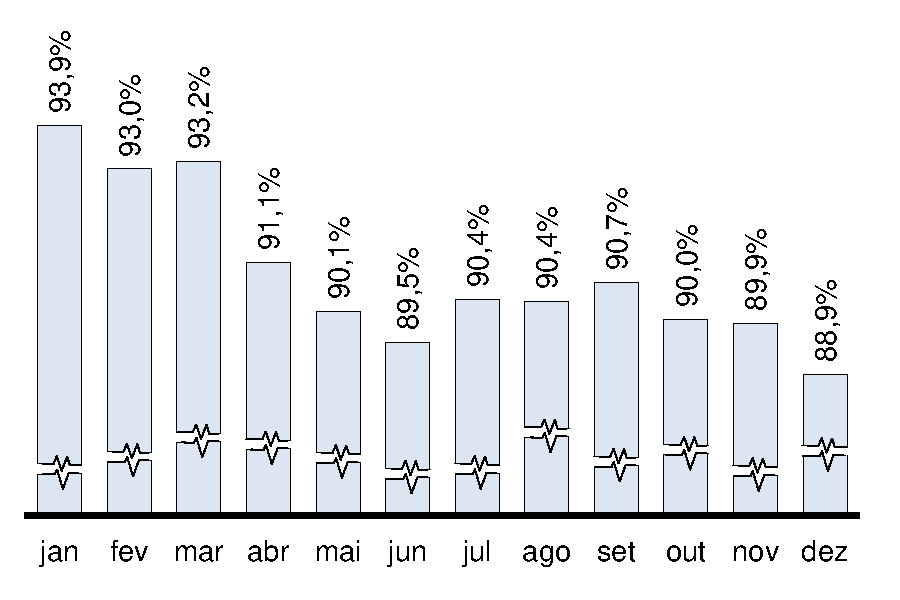
\includegraphics[scale=0.55, bb=0 0 432 288, trim=0in 0in 0in 0in]{figures/fig02-excel.pdf} %left, bottom, right and top
		\caption{Evolução do rendimento metálico na Aciaria 2 no ano de 2013\cite{rel2}.}
		\label{fig:evol_rend}
	\end{figure}		
	Num modelo de regressão, são utilizadas observações para encontrar o conjunto de fatores $a_0$ e $a_i$ que minimizam o erro quadrático médio entre os valores de $y$ e $\hat{y}$. Para avaliar a adequação do modelo as principais métricas são: o coeficiente de determinação ($r^2$) e o intervalo de confiança para as estimativas dos coeficientes. 
	
	O coeficiente de determinação representa o percentual da resposta que é explicado pelo modelo. O intervalo de confiança para as estimativas é construido com base no erro padrão (SE, \textit{standard error}) e mostra o nível de significância dos coeficientes. Se o intervalo de confiança para um coeficiente contiver o zero então não há evidência amostral para rejeitar a inexistência de relação entre a resposta e a variável explicativa.
	
	Para a criação dos modelos foi utilizando a linguagem de programação de código livre \emph{R}\cite{rcore} no ambiente \emph{R Studio}.
\section{Resultados}
	A análise exploratória dos dados foi realizada relacionando, individualmente, as variáveis explicativas ao rendimento metálico mensal.	A Tabela \ref{tab:corr} apresenta os coeficientes de determinação obtidos entre as variáveis em estudo e o rendimento metálico mensal obtidos na análise exploratória de dados.	
	\begin{table}[H]
		\begin{center}
		\begin{small}
		\caption{Análise exploratória entre as variáveis candidatas e o rendimento mensal da Aciaria 2.}
		\label{tab:corr}
			\begin{tabular}{ccc}
				\hline
				Variável & Corr. ($r$) & Det. ($r^2$) \\
				\hline \hline
				\texttt{ARET} 	& -0,0529 	&  0,0028	\\
				\texttt{PSUC}	& -0,7886	&  0,6219	\\
				\texttt{SIN.T}  &  0,9047	&  0,8185	\\
				\texttt{CB.T}	&  0,9567	&  0,9156	\\
				\texttt{PRES}	& -0,2931	&  0,0859	\\
				\texttt{PUBC}	& -0,1951	&  0,0380	\\
				\texttt{PAA}	& -0,3236	&  0,1047	\\
				\texttt{PSAGP}	& -0,7064	&  0,4990	\\
				\texttt{LIG.T}	&  0,3818	&  0,1458	\\
				\hline
			\end{tabular}
			\end{small}
			\end{center}
	\end{table}	
	Para o modelamento multivariável foram selecionados os fatores cujo coeficiente de determinação com relação ao rendimento mensal foi superior a 10\%. As Figuras de \ref{fig:psuc} a \ref{fig:ligas} apresentam o relacionamento individual entre as variáveis selecionadas e o rendimento metálico mensal. 	
	
	O primeiro modelo geral incluiu todas as variáveis selecionadas pelo critério de $r^2 > 10\%$. O coeficiente múltiplo de determinação obtido pelo modelo geral foi $r^2 = 0.97$ e o coeficiente ajustado foi $r^2_{adj}=0.93$. 
	
	A Tabela \ref{tab:mod_geral} apresenta um resumo estatístico do modelo geral de regressão múltipla.
	\begin{table}[H]
	\begin{center}
	\begin{small}
		\caption{Modelo geral de regressão linear múltipla.}
		\label{tab:mod_geral}		
			\begin{tabular}{ccccc}
				\hline
				Coef. & Estimativa & SE & t & p-valor \\
				\hline \hline
				intercepto		&  0,8162 & 0,1155 &  7,065 & 0,0009 \\
				\texttt{PSUC}	&  0,2926 & 0,3367 &  0,869 & 0,4245 \\
				\texttt{SIN.T}  &  0,0033 & 0,0035 &  0,928 & 0,3960 \\
				\texttt{CB.T}	&  0,0012 & 0,0004 &  2,780 & 0,0389 \\
				\texttt{PAA}	&  0,0001 & 0,0007 &  0,147 & 0,8890 \\
				\texttt{PSAGP}	& -0,0003 & 0,0004 & -0,767 & 0,4775 \\
				\hline
			\end{tabular}
			\end{small}
			\end{center}
	\end{table}	
	A soma dos resíduos foi $-1,0\times10^{-18}$, que é zero na precisão do computador. Além disso, a estatística AD no teste de normalidade de Anderson-Darling\cite{wiki:ad} foi 0,2337 que corresponde a um p-valor de 0,7381, grande o suficiente para falhar ao rejeitar a hipótese de normalidade.	
	
	O modelo geral mostra o nível de significância de cada fator em estudo na coluna do p-valor. Esta estatística mostra o nível de significância de um teste de hipótese no qual a hipótese nula é a de que o efeito do fator é inexistente. Portanto, são significativos apenas os fatores que tem o valor de $p$ menor que o nível de significância, $\alpha$. 
	
	Neste estudo, o nível de significância escolhido foi $\alpha = 5\%$. Foi utilizada a técnica AIC\cite{wiki:aic} (\textit{Akaike Information Criterior}) para selecionar iterativamente os melhores candidatos ao modelo linear específico. A melhor combinação utilizou como variáveis explicativas o consumo específico de ligas (\texttt{LIG.T}) e o consumo específico de sucata tipo B (\texttt{CB.T}).
	
	O resumo do modelo específo é apresentado na Tabela \ref{tab:mod_esp}. A análise do p-valor mostra que todos os coeficientes são significativos (diferentes de zero) ao nível de confiança de 95\%. O coeficiente de determinação múltiplo obtido foi $r^2=0,95$ e o valor deste coeficiente ajustado pelo tamanho da amostra foi $r_{adj}^2=0,94$. O modelo linear específico é capaz de explicar 94\% da variação do rendimento em termos de consumo de sucata tipo B e consumo de ligas.
	\begin{table}[H]
	\begin{center}
	\begin{small}
		\caption{Modelo específico de regressão linear múltipla.}
		\label{tab:mod_esp}
			\begin{tabular}{ccccc}
				\hline
				Coef. & Estimativa & SE & t & p-valor \\
				\hline \hline
				intercepto		&  0,8646  & 0,0119 &  72,575 & 9,05e-14 \\
				\texttt{CB.T}	&  0,0014  & 0,0001 &  12,626 & 4,99e-07 \\
				\texttt{LIG.T}	&  0,0030  & 0,0011 &   2,764 &    0,022 \\
				\hline
			\end{tabular}
			\end{small}
			\end{center}
	\end{table}						
	A relação entre o consumo específico de sucata tipo B foi estudado em maior profundidade. Os dados obtidos do relatório acumulado das corridas produzidas nas Aciarias por convertedor\cite{rel4} mostrou que o peso de sucata tipo B não é computado como carga sólida. Isto foi verificado para todo ano de 2013, de modo que a utilização da sucata tipo B é sempre favorável ao rendimento.
	
	A Figura \ref{fig:evol_tacb} mostra a evolução do peso utilizado de sucata tipo A e tipo B em 2013. Observa-se que a partir em abril a quantidade de sucata tipo B sobre o total de sucata recirculada passou de 91\% para 22\% e evoluiu para patamares cada vez menores. 		
	\begin{figure}[H]
		\centering
		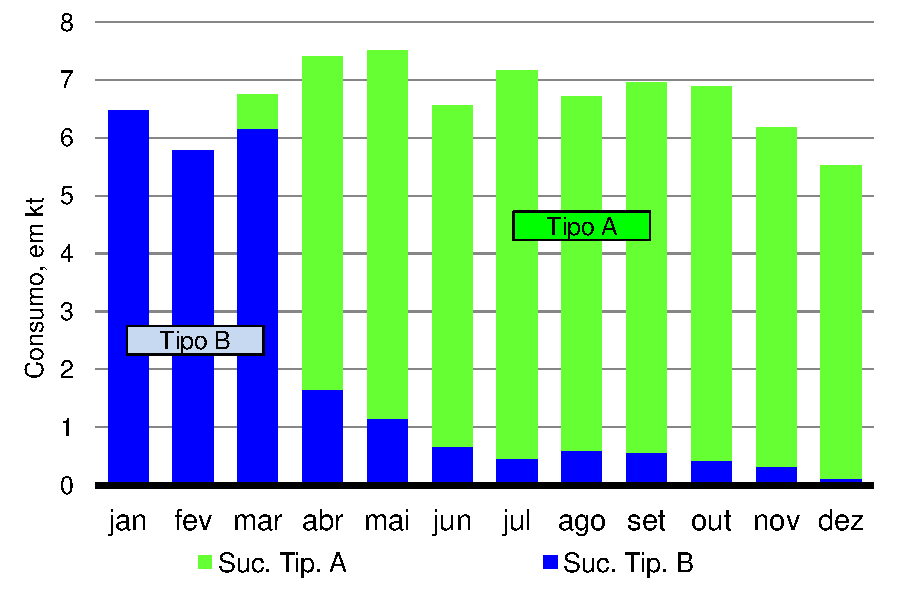
\includegraphics[scale=0.55, bb=0 0 288 432, trim=0in 0in 0in 0in]{figures/fig08-excel.pdf} %left, bottom, right and top
		\caption{Evolução mensal do consumo de sucata TA e CB\cite{rel4}.}
		\label{fig:evol_tacb}
	\end{figure}					
%%%%%%%%%%%%%%%%%%%%%%%%% This page is only for figures..
\newpage
	\begin{figure}[H]
		\centering
		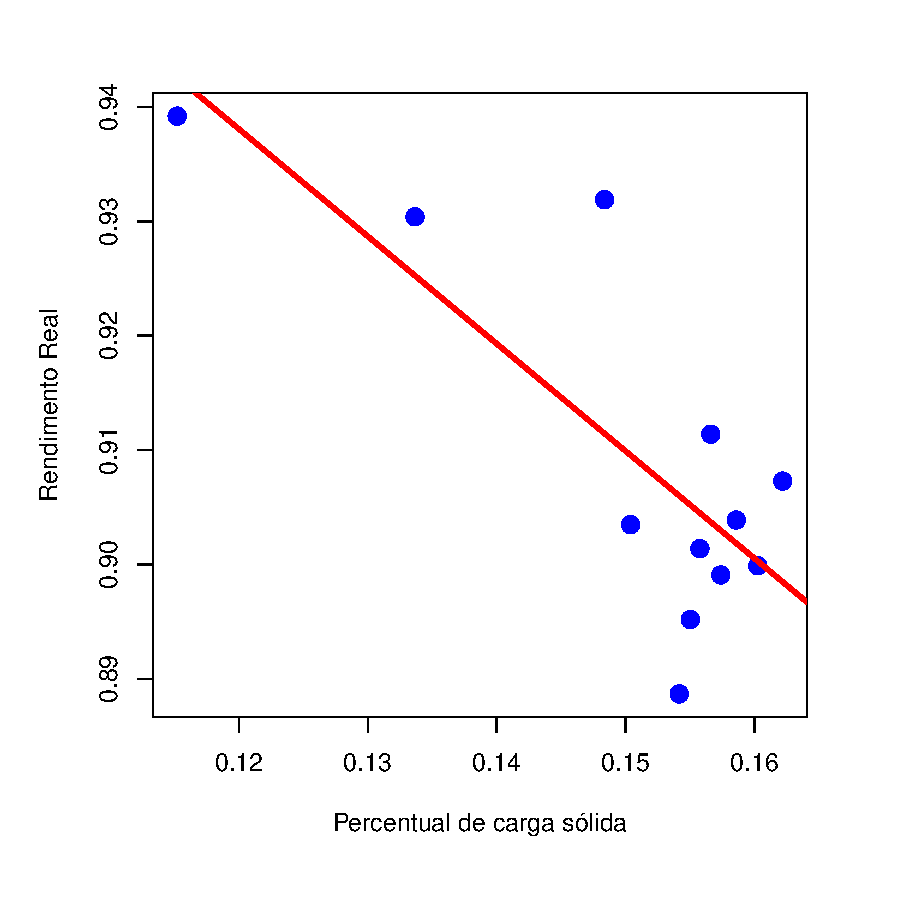
\includegraphics[scale=0.4, bb=0 0 432 432, trim=0in 0in 0in 0in]{figures/fig03.pdf} %left, bottom, right and top
		\caption{Relação entre o percentual de carga sólida e o rendimento mensal ($r^2=0,6219$).}
		\label{fig:psuc}
	\end{figure}			
	\begin{figure}[H]
		\centering
		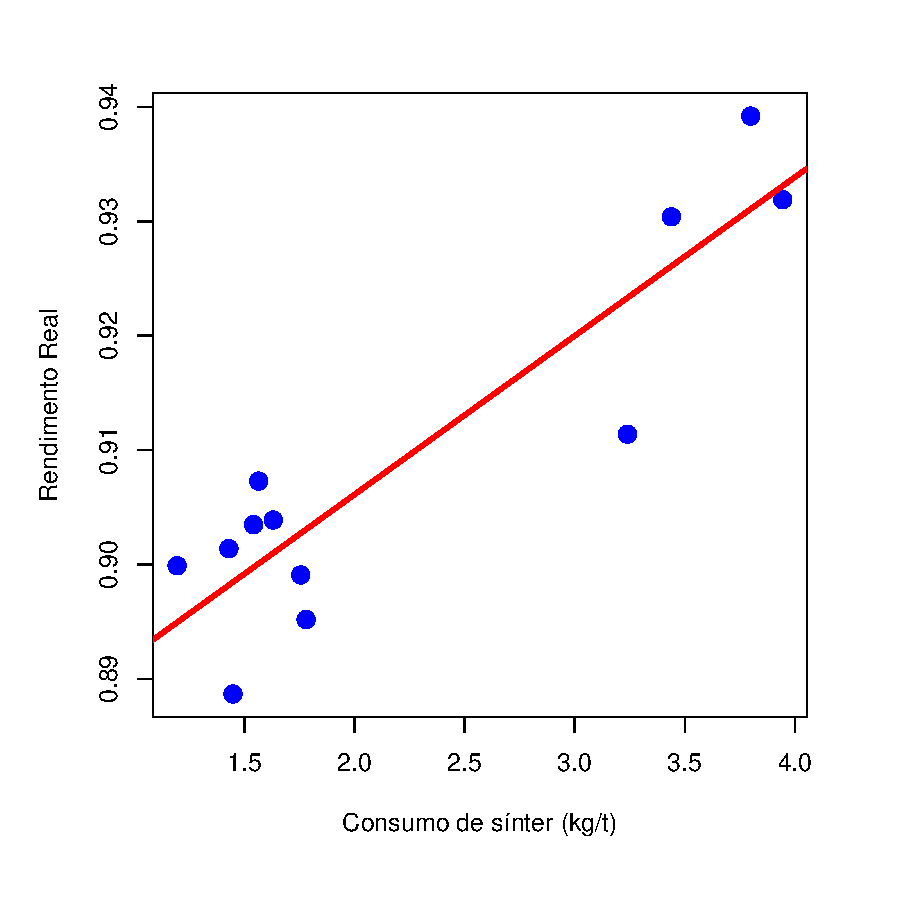
\includegraphics[scale=0.4, bb=0 0 432 432, trim=0in 0in 0in 107pt]{figures/fig04.pdf} %left, bottom, right and top
		\caption{Relação entre o consumo de sínter e o rendimento mensal ($r^2=0,8185$).}
		\label{fig:psint}
	\end{figure}
	\begin{figure}[H]
		\centering
		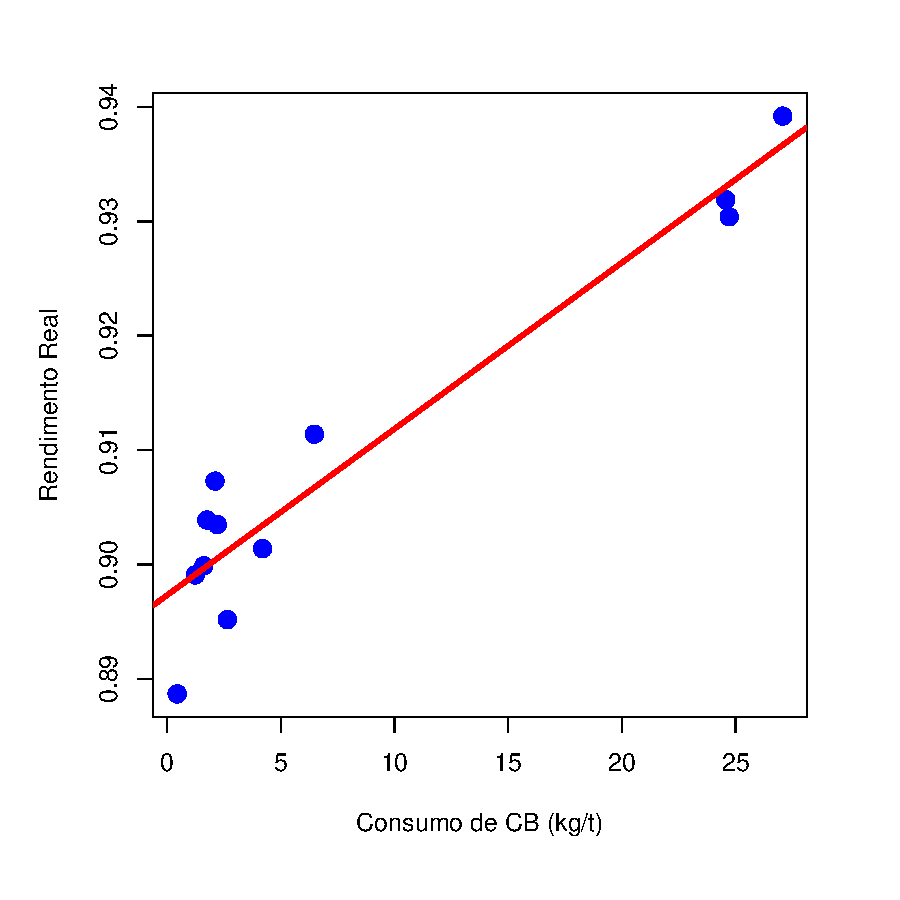
\includegraphics[scale=0.4, bb=0 0 432 432, trim=0in 0in 0in 0pt]{figures/fig05.pdf} %left, bottom, right and top
		\caption{Relação entre o consumo de CB e o rendimento mensal ($r^2=0,9156$).}
		\label{fig:cb}
	\end{figure}	
	\begin{figure}[H]
		\centering
		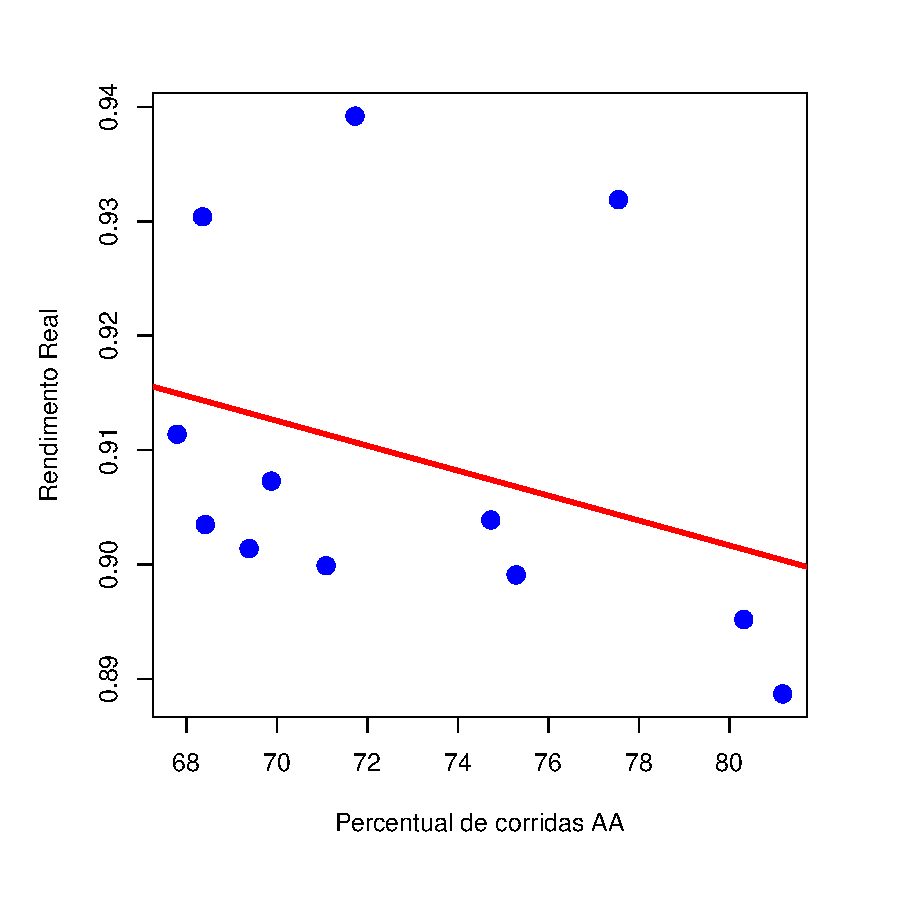
\includegraphics[scale=0.4, bb=0 0 432 432, trim=0in 0in 0in 0in]{figures/fig06.pdf} %left, bottom, right and top
		\caption{Relação entre a proporção de corridas AA e o rendimento mensal ($r^2=0,1047$).}
		\label{fig:aa}
	\end{figure}			
	\begin{figure}[H]
		\centering
		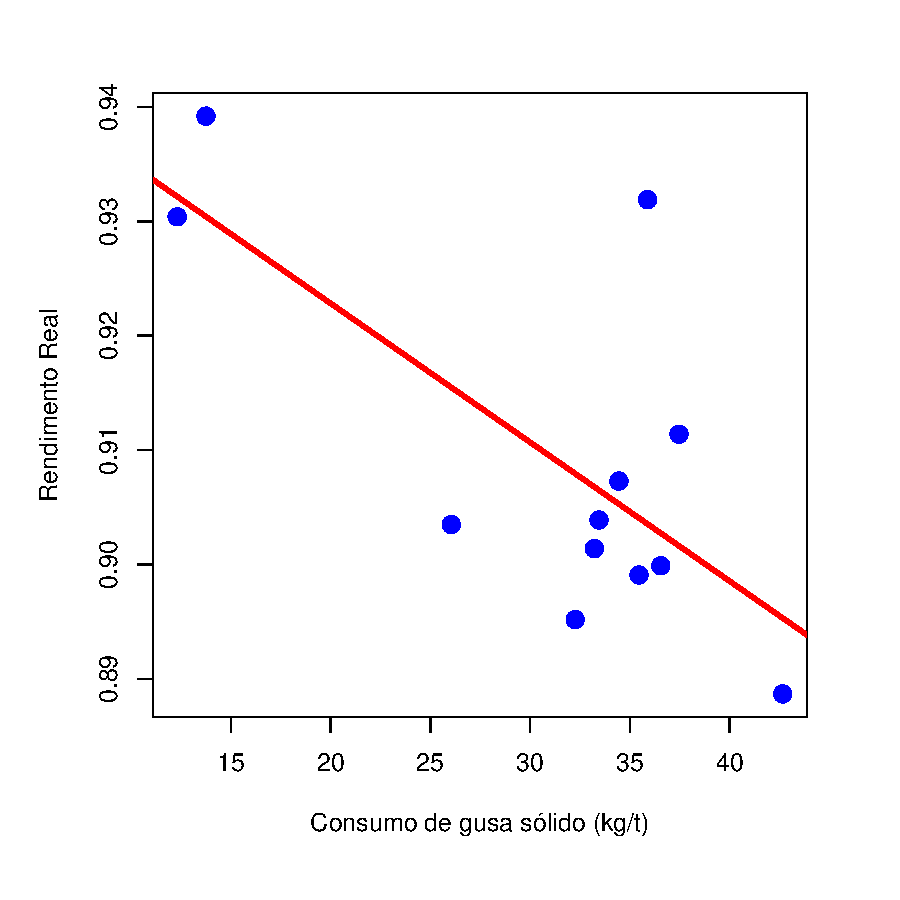
\includegraphics[scale=0.4, bb=0 0 432 432, trim=0in 0in 0in 0in]{figures/fig07.pdf} %left, bottom, right and top
		\caption{Relação entre o consumo de gusa sólido e o rendimento mensal ($r^2=0,4990$).}
		\label{fig:sagp}
	\end{figure}
	\begin{figure}[H]
		\centering
		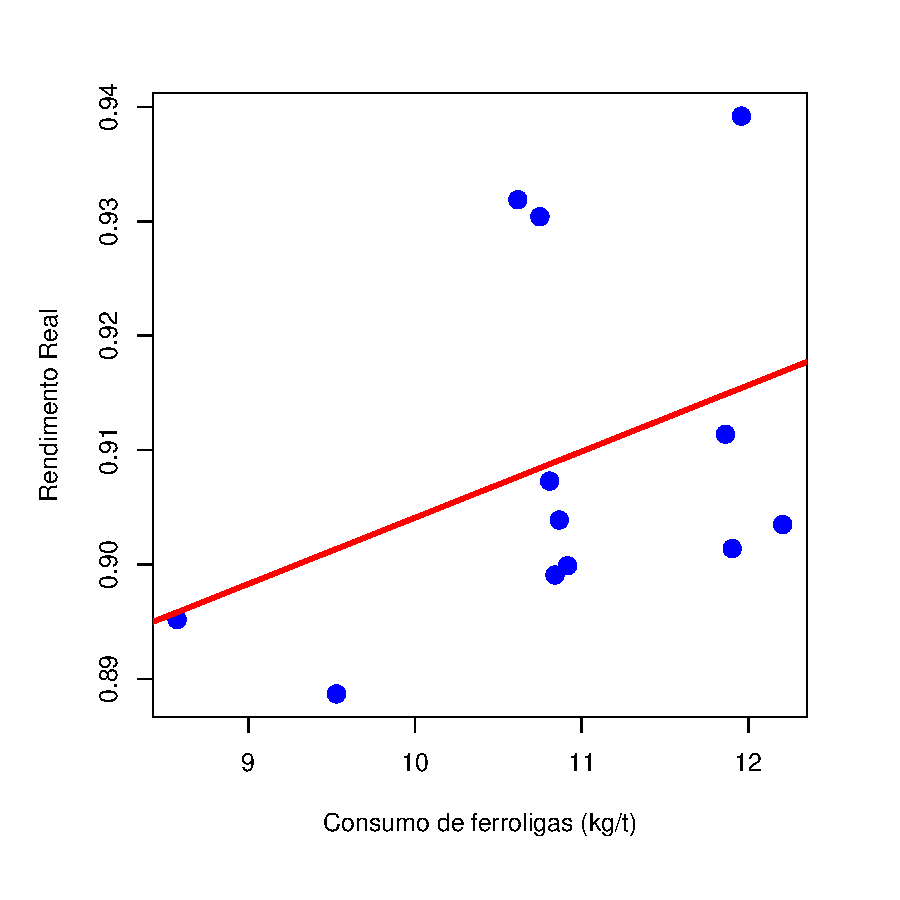
\includegraphics[scale=0.4, bb=0 0 432 432, trim=0in 0in 0in -107pt]{figures/fig10.pdf} %left, bottom, right and top
		\caption{Relação entre o consumo de ligas e o rendimento mensal ($r^2=0,3302$).}
		\label{fig:ligas}
	\end{figure}			
\newpage
	Considerando esses resultados, foi recalculado o rendimento metálico com os dados disponíveis\cite{rel4} considerando toda sucata tipo B como sucata tipo A utilizando a Equação \ref{eq:rend}. 
		
	O resultado do rendimento calculado sem o benefício da sucata tipo B é mostrado na Figura \ref{fig:new_rend}. Percebe-se que foi grande a influência da sucata CB nos primeiros meses do ano. 

	Depois de removido o efeito da contabilização de sucata recirculada, restou determinar se a variação observada no rendimento é resultado normal do processo ou se existe alguma causa especial envolvida. 
	
	Um teste de normalidade foi conduzido com os dados do rendimento corrigido (sem o efeito da sucata tipo B). O p-valor do teste de normalidade de Anderson-Darling foi 0.916, de onde se conclui que os dados distribuem-se normalmente. Em seguida, removeu-se o valor do mês de dezembro para cálculo da média ($\bar{x} = 0,9018$) e do desvio padrão ($s=0,00728$) para determinar se o rendimento de dezembro foi significativamente baixo. O valor do \emph{escore-z} foi calculado para o valor observado no mês de dezembro, utilizando a Equação \ref{eq:z}:
	\begin{equation}
		\label{eq:z}
		z = \frac{x - \bar{x}}{s} = -2,37
	\end{equation}
	O rendimento do mês de dezembro estava a 2,3 desvios-padrão da média. A probabilidade de observar um valor tão extremo quanto este é $P(z<-2,37)=3,2\%$.
	\begin{figure}[H]
		\centering
		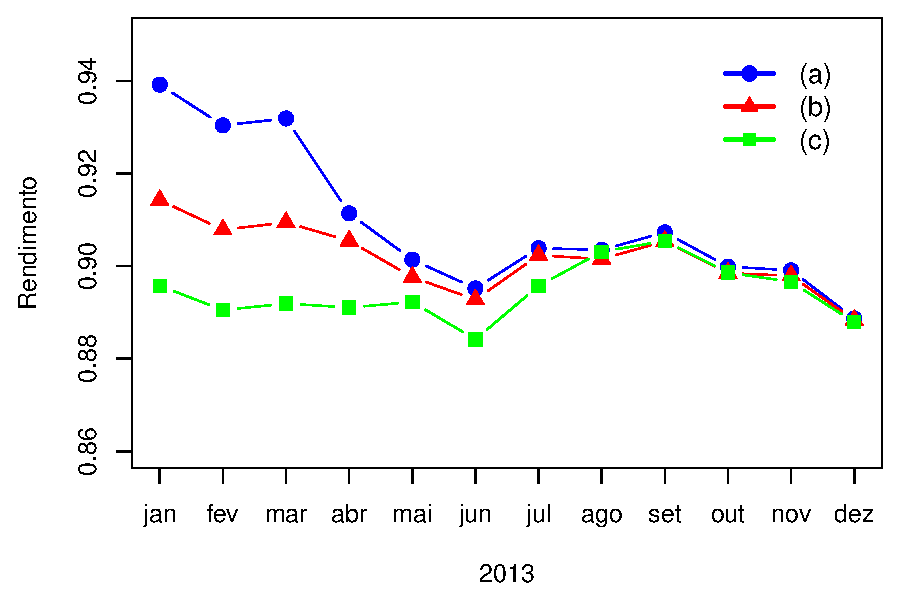
\includegraphics[scale=0.55, bb=0 0 288 432, trim=0in 0in 0in 0in]{figures/fig09.pdf} %left, bottom, right and top
		\caption{Rendimento metálico oficial\cite{rel2} e Rendimento simulado sem o efeito da sucata tipo B.}
		\label{fig:new_rend}
	\end{figure}				
	Foi construído um terceiro modelo para explicar, desta vez, o rendimento corrigido. As variáveis selecionadas pelo método AIC para explicar o rendimento sem o efeito da sucata tipo B foram o consumo específico de sínter (\texttt{CB.T}) e o consumo específico de ligas (\texttt{LIG.T}). O Resumo estatístico do modelo para o rendimento simulado é apresentado na Tabela \ref{tab:newmod}.
		\begin{table}[H]
	\begin{center}
	\begin{small}
		\caption{Modelo específico de regressão linear múltipla para o rendimento simulado.}
		\label{tab:newmod}
			\begin{tabular}{ccccc}
				\hline
				Coef. & Estimativa & SE & t & p-valor \\
				\hline \hline
				intercepto		&  0.8583 & 0.0119 &  71.878 & 9.87e-14 \\
				\texttt{SINT.T}	&  0.0048 & 0.0011 &   4.241 & 0.0022  \\
				\texttt{LIG.T}	&  0.0030 & 0.0011 &   2.698 & 0.0245  \\
				\hline
			\end{tabular}
			\end{small}
			\end{center}
	\end{table}						
	O modelo linear para explicar o rendimento sem a influência da sucata tipo B apresenta dois componentes significativos: o consumo de sínter e o consumo de ligas. Cada 1 kg/t a menos de ligas resulta numa perda de 0,30\% no rendimento, enquanto que para cada
	1 kg/t a menos de sínter o rendimento cai 0,48\%.
	
	A evolução do consumo de ligas é mostrado na Figura \ref{fig:ligas_mes}. Os menores consumos de ligas foram em junho e em dezembro, os meses em que o rendimento foi igualmente menor.
	\begin{figure}[H]
		\centering
		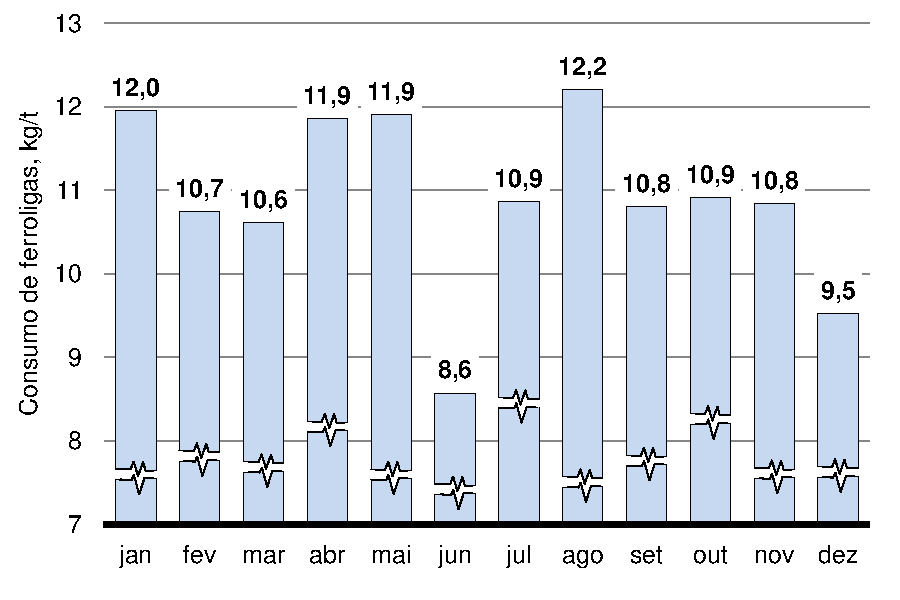
\includegraphics[scale=0.55, bb=0 0 432 288, trim=0in 0in 0in 0in]{figures/fig11-excel.pdf} %left, bottom, right and top
		\caption{Consumo mensal de ligas em kg/t\cite{rel16}.}
		\label{fig:ligas_mes}
	\end{figure}			
	Em dezembro, a diferença entre o consumo de ligas e a média dos onze primeiros meses foi de 1,5 kg/t que impactou 0,71\% no rendimento metálico. A variação do sínter foi de 0,85 kg/t, o que explica 0,26\% de perda em rendimento.
	
	Por último, foi verificado a contabilização do aço retornado. Pela Equação \ref{eq:general}, o peso de aço retornado deve ser igual ao peso de aço usado como carga metálica de modo que o efeito de ambos seja cancelado no cálculo do rendimento. Quando isso não acontece o rendimento calculado sofre influência. Quando $W_{gusaco} > W_{ret}$ a diferença entre os dois, $W_{d} = W_{gusaco}-W_{ret}$, é positiva e o denominador da Equação \ref{eq:rend} aumenta, reduzindo rendimento. 
	
	O efeito da diferença líquida ($W_{d}$) foi averiguado e em nenhum período de 2013 o rendimento foi influenciado pela diferença de aços retornados em pelo menos 0,1\%.
\section{Conclusões}
	Modelamento estatístico foi conduzido utilizando regressão linear multivariada para identificar os fatores que explicam a queda observada no rendimento metálico da Aciaria 2. O efeito da substituição da sucata tipo B pela tipo A foi removido pela criação de um rendimento simulado. 
	
	O efeito da diferença eventual entre o aço retornado informado pelo lingotamento e o carregado pelo convertedor mostrou-se irrelevante, nunca chegando a 0,1\%.
	
	O rendimento sem efeito da sucata tipo A foi modelado em função do consumo de sínter e do consumo de ligas. O efeito no rendimento, por kg/t, foi de 0,30\% para as ligas e 0,48\% para o sínter.
	
	A variação de rendimento explicada por ligas e sínter no mes de dezembro foi de 1,11\%.
%%%%%%%%%%%%%%%%%%%%%%%%%%%%%%%%%%%%%%%%%%%%%%%%%%%%%%
\bibliographystyle{IEEE/abntex2-num}
% \bibliographystyle{IEEE/IEEEtranN}
% \bibliographystyle{plainnat}
% enable it only if you want to display some
% this command renames the reference section: http://tex.stackexchange.com/questions/12597/renaming-the-bibliography-page-using-bibtex
\renewcommand{\bibname}{Referências}
\bibliography{references}

\end{multicols}	